\hypertarget{GUIRenderCutCanvas_8cpp}{\section{simpleanalyzer-\/gui/src/\-G\-U\-I/\-G\-U\-I\-Render\-Cut\-Canvas.cpp-\/\-Dateireferenz}
\label{GUIRenderCutCanvas_8cpp}\index{simpleanalyzer-\/gui/src/\-G\-U\-I/\-G\-U\-I\-Render\-Cut\-Canvas.\-cpp@{simpleanalyzer-\/gui/src/\-G\-U\-I/\-G\-U\-I\-Render\-Cut\-Canvas.\-cpp}}
}
{\ttfamily \#include \char`\"{}G\-U\-I\-Render\-Cut\-Canvas.\-h\char`\"{}}\\*
{\ttfamily \#include \char`\"{}G\-U\-I\-Cut\-Render\-Window.\-h\char`\"{}}\\*
{\ttfamily \#include $<$vector$>$}\\*
{\ttfamily \#include \char`\"{}../processing/utils.\-h\char`\"{}}\\*
{\ttfamily \#include \char`\"{}../processing/\-Object\-Data.\-h\char`\"{}}\\*
{\ttfamily \#include \char`\"{}G\-U\-I\-Main\-Window.\-h\char`\"{}}\\*
{\ttfamily \#include \char`\"{}Renderer.\-h\char`\"{}}\\*
{\ttfamily \#include $<$iostream$>$}\\*
Include-\/\-Abhängigkeitsdiagramm für G\-U\-I\-Render\-Cut\-Canvas.\-cpp\-:
\nopagebreak
\begin{figure}[H]
\begin{center}
\leavevmode
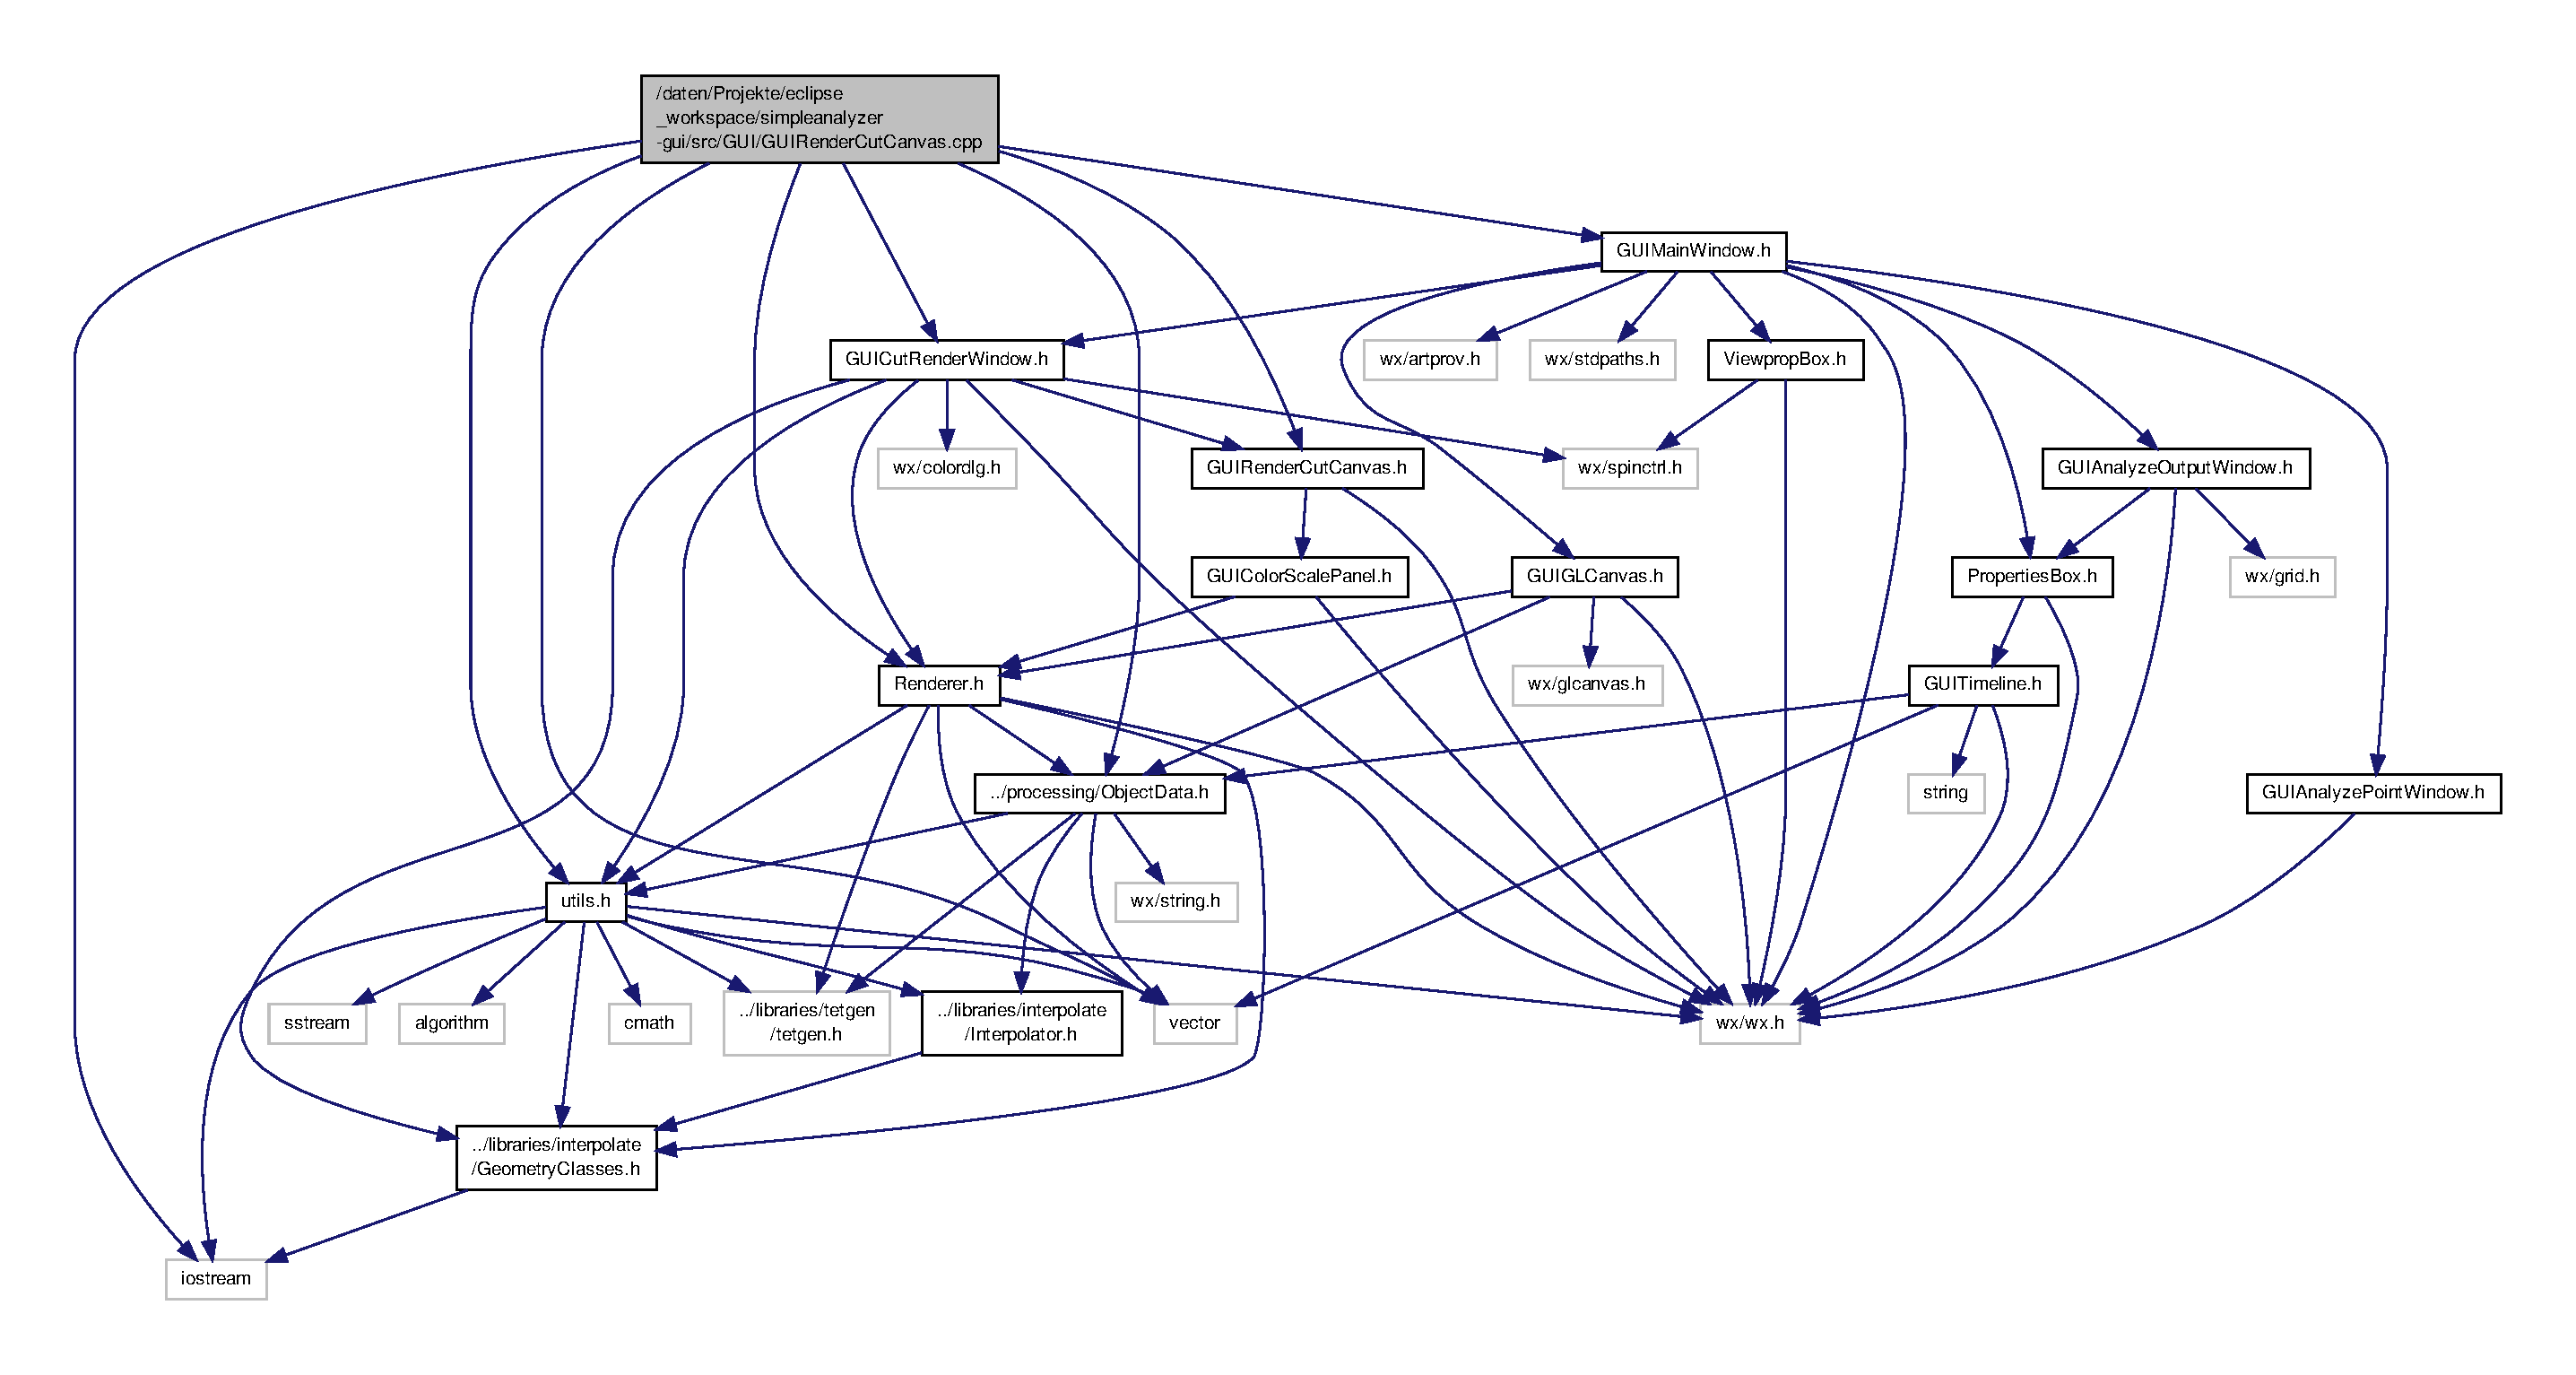
\includegraphics[width=350pt]{GUIRenderCutCanvas_8cpp__incl}
\end{center}
\end{figure}
